\documentclass[12pt]{article}
\usepackage{amsmath}
\usepackage{graphicx}
\usepackage{hyperref}
\usepackage{listings}
\usepackage{color}
\usepackage{pythonhighlight}

\title{Operating System Course Report - First Half of the Semester}
\author{A class}
\date{\today}

\begin{document}

\maketitle
\newpage

\tableofcontents
\newpage

\section{Introduction}
This report summarizes the topics covered during the first half of the Operating System course. It includes theoretical concepts, practical implementations, and assignments. The course focuses on the fundamentals of operating systems, including system architecture, process management, CPU scheduling, and deadlock handling.

\section{Course Overview}
\subsection{Objectives}
The main objectives of this course are:
\begin{itemize}
    \item To understand the basic components and architecture of a computer system.
    \item To learn process management, scheduling, and inter-process communication.
    \item To explore file systems, input/output management, and virtualization.
    \item To study the prevention and handling of deadlocks in operating systems.
\end{itemize}

\subsection{Course Structure}
The course is divided into two halves. This report focuses on the first half, which covers:
\begin{itemize}
    \item Basic Concepts and Components of Computer Systems
    \item System Performance and Metrics
    \item System Architecture of Computer Systems
    \item Process Description and Control
    \item Scheduling Algorithms
    \item Process Creation and Termination
    \item Introduction to Threads
    \item File Systems
    \item Input and Output Management
    \item Deadlock Introduction and Prevention
    \item User Interface Management
    \item Virtualization in Operating Systems
\end{itemize}

\section{Topics Covered}

\subsection{Basic Concepts and Components of Computer Systems}
This section explains the fundamental components that make up a computer system, including the CPU, memory, storage, and input/output devices.

\subsection{System Performance and Metrics}
This section introduces various system performance metrics used to measure the efficiency of a computer system, including throughput, response time, and utilization.

\subsection{System Architecture of Computer Systems}
Describes the architecture of modern computer systems, focusing on the interaction between hardware and the operating system.

\subsection{Process Description and Control}
Processes are a central concept in operating systems. This section covers:
\begin{itemize}
    \item Process states and state transitions
    \item Process control block (PCB)
    \item Context switching
\end{itemize}

\subsection{Scheduling Algorithms}
This section covers:
\begin{itemize}
    \item First-Come, First-Served (FCFS)
    \item Shortest Job Next (SJN)
    \item Round Robin (RR)
\end{itemize}
It explains how these algorithms are used to allocate CPU time to processes.

\subsection{Process Creation and Termination}
Details how processes are created and terminated by the operating system, including:
\begin{itemize}
    \item Process spawning
    \item Process termination conditions
\end{itemize}

\subsection{Introduction to Threads}
This section introduces the concept of threads and their relation to processes, covering:
\begin{itemize}
    \item Single-threaded vs. multi-threaded processes
    \item Benefits of multithreading
\end{itemize}

\begin{figure}[h]
    \centering
    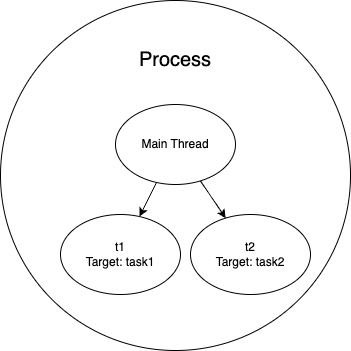
\includegraphics[width=0.5\textwidth]{/Users/khawaritzmi/Unhas/os_report_mid2024/a_class/asset/example.png}  % Sesuaikan nama file dan ukurannya
    \caption{Ini adalah gambar contoh dari multithreading.}
    \label{fig:contoh_gambar}
\end{figure}

Seperti yang terlihat pada Gambar \ref{fig:contoh_gambar}, inilah cara menambahkan gambar dengan keterangan.

\subsection{File Systems}
File systems provide a way for the operating system to store, retrieve, and manage data. This section explains:
\begin{itemize}
    \item File system concept
    File adalah unit penyimpanan logis yang diabstraksikan oleh sistem operasi dari perangkat penyimpanan. File berisi informasi yang disimpan di penyimpanan sekunder (seperti disk magnetik, pita magnetik, dan disk optik). Informasi dalam file ditentukan oleh pembuatnya. Sebuah file memiliki struktur tertentu tergantung pada jenisnya. Jenis file terdiri dari data numerik, karakter, dan biner, serta program seperti program sumber, program objek, dan program yang dapat dieksekusi.
    
    Atribut file 

    Sebuah file memiliki atribut yang bervariasi dari satu sistem operasi ke sistem operasi lainnya, tetapi umumnya terdiri dari file : 

    - Nama, informasi yang disimpan dalam bentuk yang dapat dibaca manusia  
    
    - Jenis, diperlukan untuk sistem yang mendukung berbagai jenis. 
    
     - Lokasi, penunjuk lokasi file pada perangkat. 
    
     - Ukuran, ukuran file saat ini. 
    
     - Perlindungan, mengontrol siapa yang dapat membaca, menulis, dan menjalankan. 
    
      - Waktu, tanggal dan identifikasi pengguna, data untuk memantau perlindungan, keamanan dan penggunaan. 

        Informasi file disimpan dalam struktur direktori yang diatur berdasarkan disk. 
    
        Operasi pada file 
    
             	Sebagai tipe data abstrak, perlu untuk mendefinisikan operasi yang dapat dibentuk oleh file. Ada enam operasi dasar yang disediakan sebagai panggilan sistem, yaitu: 
    
     		- Membuat file (create)  
    
     		- Menulis file (write)  
    
     		- Membaca file (read) 
    
     		- Mencari kembali file (file seek) 
    
     		- Menghapus file (delete) 
    
        	- Memotong file (truncate)  
    
        	- Open(Fi) mencari struktur direktori untuk entri Fi dan memindahkan isi entri ke memori. 
    
     		- Close(Fi) memindahkan isi entri Fi dalam memori ke struktur direktori pada disk. 
     		   Operasi tambahan yang biasanya dilakukan pada file 
                  adalah: 
    
     		- Menambahkan (append) informasi baru pada akhir file yang sudah ada 
    
     		- Mengganti nama file yang sudah ada 
    
     		- Menggandakan (menyalin) file
       
                \begin{figure}[h]
                            \centering
                            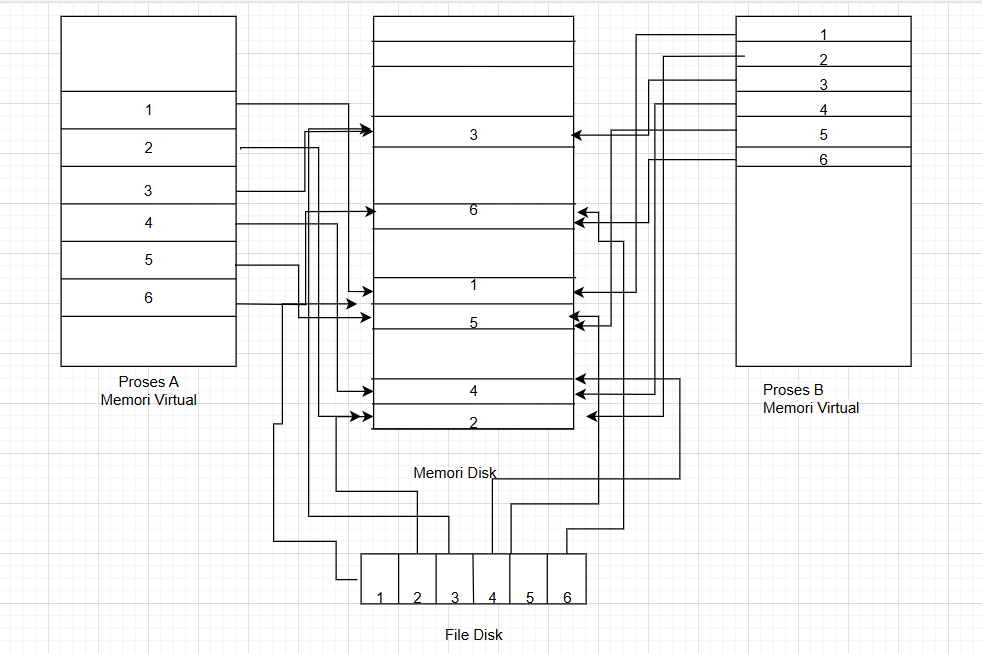
\includegraphics[width=0.5\linewidth]
                            {asset/gambarfilesystem.png}
                            \caption{Contoh Pemetaan File ke Memori}
                            \label{fig:deadlock-RAG}
                            \end{figure}
       
              Sebagian besar operasi file melibatkan pencarian direktori untuk input yang terkait dengan file. Untuk menghindari pencarian yang tetap, beberapa sistem akan membuka file saat pertama kali aktif. Sistem operasi menyimpan tabel kecil yang berisi informasi tentang semua file yang terbuka (tabel file terbuka). Ketika file tidak lagi digunakan, file akan ditutup oleh proses dan sistem operasi akan menghapus file tersebut dari tabel file terbuka. Beberapa informasi yang terkait dengan pembukaan file adalah: 
    
     		 - Penunjuk file. 
    
     		 - Jumlah file yang dibuka. 
    
     		 - Lokasi file pada disk. 
    
      Jenis file 
      Salah satu pertimbangan penting dalam mendesain sistem berkas dan keseluruhan sistem operasi adalah apakah sistem operasi mengenali dan mendukung sistem berkas. Jika sistem operasi mengenali jenis file, maka operasi dapat dilakukan pada file dengan cara yang rasional. Sebagai contoh, pengguna yang mencoba mencetak file yang dapat dieksekusi dapat dicegah oleh sistem operasi karena file tersebut adalah program biner. Teknik umum untuk mengimplementasikan tipe file adalah dengan menyertakan tipe file sebagai bagian dari nama file. Nama file dibagi menjadi dua bagian: nama dan ekstensi (seperti pada MS-DOS) seperti yang ditunjukkan pada Gambar 9-2. Setiap file memiliki atribut pembuat yang berisi nama program yang membuatnya (seperti pada MSWindows/Apple Macintosh). Atribut ini diatur oleh sistem operasi ketika menggunakan panggilan sistem create. Ketika pengguna membuka file dengan mengklik dua kali mouse pada ikon file, program yang dibuat akan ditampilkan secara otomatis. UNIX menggunakan nomor ajaib yang disimpan di awal file untuk menunjukkan jenis file seperti program yang dapat dieksekusi, file batch (shell script), file postscript dan lain-lain. Tidak semua file mempunyai magic number, sehingga informasi tipe tidak dapat dijelaskan. UNIX tidak menyimpan nama program yang membuatnya. UNIX juga mengijinkan nama ekstensi file disembunyikan, sehingga user dapat menentukan sendiri jenis file dan tidak tergantung pada sistem operasi. 

      Struktur file 
      Jenis file juga digunakan untuk menunjukkan struktur internal file. File tertentu harus mengonfirmasi struktur yang diperlukan yang dipahami oleh sistem operasi. Misalnya, sistem operasi memerlukan file yang dapat dieksekusi yang memiliki struktur khusus sehingga dapat menentukan di mana letak memori dan lokasi instruksi pertama. Beberapa sistem operasi menggunakan seperangkat sistem pendukung struktur file dengan sejumlah operasi khusus untuk memanipulasi file dengan struktur ini. Ini merupakan kelemahan dalam sistem operasi yang mendukung lebih dari satu struktur file. Jika sistem operasi menetapkan 10 struktur file yang berbeda, sistem operasi perlu menyertakan kode untuk mendukung struktur file tersebut. Setiap file harus didefinisikan sebagai salah satu jenis file yang didukung oleh sistem operasi. Beberapa sistem operasi seperti UNIX dan MS-DOS hanya mendukung sejumlah struktur file yang terbatas. UNIX mendefinisikan setiap berkas sebagai urutan byte 8 bit dan bit-bit ini tidak diterjemahkan oleh sistem operasi. Skema ini memiliki fleksibilitas maksimum, tetapi sedikit dukungan. Setiap program aplikasi harus menyertakan kodenya sendiri untuk menerjemahkan file input ke dalam struktur yang benar. Semua SO harus mendukung setidaknya satu struktur file yang dapat dieksekusi sehingga sistem dapat memuat dan menjalankan program. 

      Struktur file internal 
      Jenis file 

      Salah satu pertimbangan penting dalam mendesain sistem berkas dan keseluruhan sistem operasi adalah apakah sistem operasi mengenali dan mendukung sistem berkas. Jika sistem operasi mengenali jenis file, maka operasi dapat dilakukan pada file dengan cara yang rasional. Sebagai contoh, pengguna yang mencoba mencetak file yang dapat dieksekusi dapat dicegah oleh sistem operasi karena file tersebut adalah program biner. Teknik umum untuk mengimplementasikan tipe file adalah dengan menyertakan tipe file sebagai bagian dari nama file. Nama file dibagi menjadi dua bagian: nama dan ekstensi (seperti pada MS-DOS) seperti yang ditunjukkan pada Gambar 9-2. Setiap file memiliki atribut pembuat yang berisi nama program yang membuatnya (seperti pada MSWindows/Apple Macintosh). Atribut ini diatur oleh sistem operasi ketika menggunakan panggilan sistem create. Ketika pengguna membuka file dengan mengklik dua kali mouse pada ikon file, program yang dibuat akan ditampilkan secara otomatis. UNIX menggunakan nomor ajaib yang disimpan di awal file untuk menunjukkan jenis file seperti program yang dapat dieksekusi, file batch (shell script), file postscript dan lain-lain. Tidak semua file mempunyai magic number, sehingga informasi tipe tidak dapat dijelaskan. UNIX tidak menyimpan nama program yang membuatnya. UNIX juga mengijinkan nama ekstensi file disembunyikan, sehingga user dapat menentukan sendiri jenis file dan tidak tergantung pada sistem operasi. 

      Struktur file 
      Jenis file juga digunakan untuk menunjukkan struktur internal file. File tertentu harus mengonfirmasi struktur yang diperlukan yang dipahami oleh sistem operasi. Misalnya, sistem operasi memerlukan file yang dapat dieksekusi yang memiliki struktur khusus sehingga dapat menentukan di mana letak memori dan lokasi instruksi pertama. Beberapa sistem operasi menggunakan seperangkat sistem pendukung struktur file dengan sejumlah operasi khusus untuk memanipulasi file dengan struktur ini. Ini merupakan kelemahan dalam sistem operasi yang mendukung lebih dari satu struktur file. Jika sistem operasi menetapkan 10 struktur file yang berbeda, sistem operasi perlu menyertakan kode untuk mendukung struktur file tersebut. Setiap file harus didefinisikan sebagai salah satu jenis file yang didukung oleh sistem operasi. Beberapa sistem operasi seperti UNIX dan MS-DOS hanya mendukung sejumlah struktur file yang terbatas. UNIX mendefinisikan setiap berkas sebagai urutan byte 8 bit dan bit-bit ini tidak diterjemahkan oleh sistem operasi. Skema ini memiliki fleksibilitas maksimum, tetapi sedikit dukungan. Setiap program aplikasi harus menyertakan kodenya sendiri untuk menerjemahkan file input ke dalam struktur yang benar. Semua SO harus mendukung setidaknya satu struktur file yang dapat dieksekusi sehingga sistem dapat memuat dan menjalankan program. 
    \item File system structure
    \item File access methods
    \item Directory management
\end{itemize}

\subsection{Input and Output Management}
Input and output management is key for handling the interaction between the system and external devices. This section includes:
\begin{itemize}
    \item Device drivers
    \item I/O scheduling
\end{itemize}

\subsection{Deadlock Introduction and Prevention}
Explores the concept of deadlocks and methods for preventing them:
\begin{itemize}
    \item Deadlock conditions
    \item Deadlock prevention techniques
\end{itemize}

\subsection{User Interface Management}
This section discusses the role of the operating system in managing the user interface. Topics covered include:
\begin{itemize}
    \item Graphical User Interface (GUI)
    \item Command-Line Interface (CLI)
    \item Interaction between the user and the operating system
\end{itemize}

\subsection{Virtualization in Operating Systems}
Virtualization allows multiple operating systems to run concurrently on a single physical machine. This section explores:
\begin{itemize}
    \item Concept of virtualization
    \item Hypervisors and their types
    \item Benefits of virtualization in modern computing
\end{itemize}

\section{Assignments and Practical Work}
\subsection{Assignment 1: Process Scheduling}
Students were tasked with implementing various process scheduling algorithms (e.g., FCFS, SJN, and RR) and comparing their performance under different conditions.
\subsubsection{Group 1}
\begin{python}
    class Process:
    def __init__(self, pid, arrival_time, burst_time):
        self.pid = pid
        self.arrival_time = arrival_time
        self.burst_time = burst_time
        self.completion_time = 0
        self.turnaround_time = 0
        self.waiting_time = 0
\end{python}

\begin{table}[htbp] % Optional: For floating position
    \centering
    \begin{tabular}{|c|c|c|} % Defines number of columns and alignment (c = center, l = left, r = right). '|' creates vertical lines.
    \hline
    Header 1 & Header 2 & Header 3 \\ % Column headers
    \hline
    Row 1, Column 1 & Row 1, Column 2 & Row 1, Column 3 \\ % First row of data
    \hline
    Row 2, Column 1 & Row 2, Column 2 & Row 2, Column 3 \\ % Second row of data
    \hline
    \end{tabular}
    \caption{Your table caption} % Optional: For adding a caption
    \label{tab:your_label} % Optional: For cross-referencing the table
\end{table}
\subsection{Assignment 2: Deadlock Handling}
In this assignment, students were asked to simulate different deadlock scenarios and explore various prevention methods.

\subsection{Assignment 3: Multithreading and Amdahl's Law}
This assignment involved designing a multithreading scenario to solve a computationally intensive problem. Students then applied **Amdahl's Law** to calculate the theoretical speedup of the program as the number of threads increased.

\subsection{Assignment 4: Simple Command-Line Interface (CLI) for User Interface Management}
Students were tasked with creating a simple **CLI** for user interface management. The CLI should support basic commands such as file manipulation (creating, listing, and deleting files), process management, and system status reporting.

\subsection{Assignment 5: File System Access}
In this assignment, students implemented file system access routines, including:
\begin{itemize}
    \item File creation and deletion
    \item Reading from and writing to files
    \item Navigating directories and managing file permissions
\end{itemize}

\section{Conclusion}
The first half of the course introduced core operating system concepts, including process management, scheduling, multithreading, and file system access. These topics provided a foundation for more advanced topics to be covered in the second half of the course.

\end{document}